\documentclass[10pt,twocolumn,letterpaper]{article}

\usepackage{cvpr}
\usepackage{times}
\usepackage{epsfig}
\usepackage{graphicx}
\usepackage{amsmath}
\usepackage{amssymb}
%%%%%%%%%%% CVPR template packages end %%%%%%%%%%%%%%
\usepackage{verbatim} % for comment environment
% \usepackage{soul} % for \hl highlighting
% Include other packages here, before hyperref.

% If you comment hyperref and then uncomment it, you should delete
% egpaper.aux before re-running latex.  (Or just hit 'q' on the first latex
% run, let it finish, and you should be clear).
\usepackage[pagebackref=true,breaklinks=true,letterpaper=true,colorlinks,bookmarks=false]{hyperref}

%\cvprfinalcopy % *** Uncomment this line for the final submission

\def\cvprPaperID{489} % *** Enter the CVPR Paper ID here
\def\httilde{\mbox{\tt\raisebox{-.5ex}{\symbol{126}}}}

% 3D pose of the cars and ego motion
\newcommand{\pos}[2]{\mathbf{p}^{(#1)}(#2)}
\newcommand{\ori}[2]{\mathbf{\omega}^{(#1)}(#2)}
\newcommand{\state}[2]{\mathbf{s}^{#1}(#2)}

% ego pose
\newcommand{\egop}[1][t]{\pos{c}{#1}}
\newcommand{\egoo}[1][t]{\ori{c}{#1}}
\newcommand{\egos}[1][t]{\state{c}{#1}}

% relative pose between camera and car $i$
\newcommand{\relp}[2]{\Omega^{#1}(#2)}
\newcommand{\relpz}[2]{\Omega_z^{#1}(#2)}

% 3D tracks on car $i$ in its own coordinate frame
\newcommand{\tracklets}{\mathbf{X}^{(i)}_o}
\newcommand{\tracklet}[1]{\mathbf{x}^{(i)}_{#1}}
% track projections on camera
\newcommand{\trackp}[1]{\mathbf{u}^{(i)}(#1)}
\newcommand{\trackpj}[1]{\mathbf{u}_j(#1)}
% Unclassified track point projected on camera
\newcommand{\ucTrackp}{\mathbf{u}(t)}


% dimensions of car $i$
\newcommand{\dimsn}[1]{\mathbf{B}^{#1}}
\newcommand{\expDimsn}{\hat{\mathbf{B}}}

% projection function
\newcommand{\projectionOf}[1]{\pi_{\relp{i}{t}}\left(#1\right)}
\newcommand{\projectionOft}[1]{\pi_{\relp{i}{t+1}}\left(#1\right)}
\newcommand{\centerProj}{\bar{\pi}_{\relp{i}{t}}(\dimsn{i})}
\newcommand{\cornerProj}[1]{\pi^{#1}_{\relp{i}{t}}(\dimsn{i})}
\newcommand{\triangleProj}[1]{\triangle^{#1}_{\relp{i}{t}}(\dimsn{i})}

% bounding box corners on image
\newcommand{\bb}[1]{\mathbf{d}^{#1}(t)}

\newcommand{\Energy}[1]{\mathcal{E}^{it}_{\text{#1}}}
\newcommand{\pEnergy}[1]{\mathcal{E}^{ijt}_{\text{#1}}}
% Weighted energy
\newcommand{\WEnergy}[1]{\lambda_{\text{#1}}\Energy{#1}}
\newcommand{\EnergyCol}{\mathcal{E}^{ijt}_{\text{col}}}
\newcommand{\WEnergyCol}{\lambda_{\text{col}}\EnergyCol}

\newcommand{\occFreeProj}[1]{\Pi_{\relp{i}{t}}(#1)}
\newcommand{\minx}{x_{\text{min}}}
\newcommand{\miny}{y_{\text{min}}}
\newcommand{\maxx}{x_{\text{max}}}
\newcommand{\maxy}{y_{\text{max}}}
\newcommand{\frontface}{F^i_\text{FF}(t)}

\newcommand{\occ}[1]{o({#1})}
\newcommand{\face}{F^i_k(t)}

\newcommand{\invProjectionOf}[1]{\pi^{-1}_{\relp{i}{t}}\left(#1\right)}
\newcommand{\occf}{f^i_{occ}(\mathbf{x}_j)}
\newcommand{\occftot}{f_{occ}(\mathbf{x}_j)}
\newcommand{\occft}[1]{f_{occ}(#1)}

\newcommand{\ray}{\hat{\mathbf{r}}_j}
\newcommand{\occfray}{f_{occ}(\lambda\ray)}
\newcommand{\lambdadist}{f_{\lambda}(\trackpj{t-1}, \lambda)}

\newcommand{\occfxi}{L(\mathbf{x}; \pos{i}{t-1}, \Sigma_i)}
\newcommand{\occfi}{L(\lambda \ray; \pos{i}{t-1}, \Sigma_i)}
\newcommand{\assocP}{a^{(ij)}(\lambda)}
\newcommand{\assocPk}{a^{(ij)}(\lambda_k)}

\newcommand{\Ereproj}{E^{(ij)}_{\text{reproj}}}
\newcommand{\Ptrans}{P^{(j)}_{\text{transmission}}(\lambda)}
\newcommand{\Ptransmud}{P^{(j)}_{\text{transmission}}(\mu^{(i)}_d)}
\newcommand{\Prefl}{P^{(ij)}_{\text{reflection}}(\lambda)}
\newcommand{\dishort}{d_i(\mathbf{x})}

\newcommand{\Lu}{L_u(\mathbf{u}, \mu^i_u,\Sigma^i_u)}
\newcommand{\Llambda}{L_{\lambda}(\mathbf{u}, \lambda; \mu^i_d)}

\newcommand{\Gauss}{\mathcal{N}}
\newcommand{\PropDist}{\mathcal{W}_j}

\newcommand{\muijl}{\mu^{(ij)}_{\lambda}}
\newcommand{\sigmaijl}{\sigma^{ij}_{\lambda}}

\newcommand{\Sigmait}{\Sigma^{(i)^{-1}}_t}

\newcommand{\muit}{\mu^(i)_t}
\newcommand{\Sigmaic}{\Sigma'^{(i)^{-1}}_c}

\newcommand{\muic}{{\mu^(i)_c}}
\newcommand{\Sigmaicf}{\Sigma^{(i)^{-1}}_c}

\newcommand{\muiu}{\mu^{(i)}_t}
\newcommand{\Sigmaiu}{\Sigma^{(i)^{-1}}_u}

\newcommand{\xt}{\mathbf{x}_t}
\newcommand{\xc}{\mathbf{x}_c}

\newcommand{\Rctot}{R}
\newcommand{\tctot}{t}

\newcommand{\tcmut}{t'}


\newcommand{\Beizer}{B\'eizer }

\newcommand{\LaneUncertainty}[1]{\Sigma_{L_m}(#1)}
\newcommand{\projOnLane}[1]{\pi_{L_m(k)}(#1)}

% Pages are numbered in submission mode, and unnumbered in camera-ready
%\ifcvprfinal\pagestyle{empty}\fi
%\setcounter{page}{4321}
%\DeclareMathSymbol{\Tangent}
\DeclareMathOperator{\sech}{sech}
\DeclareMathOperator{\poly}{poly}
\DeclareMathOperator*{\argmin}{\arg\min}

\begin{document}
\title{Continuous Models for Scene and Traffic Participant Interactions in Road Scene Understanding.}
\author{Vikas Dhiman\\
  University of Michigan\\
  Ann Arbor, MI, USA\\
{\tt\small dhiman@umich.edu}
\and
Manmohan Chandraker\\
NEC Laboratories America, Inc.\\
Cupertino, CA, USA\\
{\tt\small manu@nec-labs.com}
\and
Jason J Corso\\
  University of Michigan\\
  Ann Arbor, MI, USA\\
{\tt\small jjcorso@eecs.umich.edu}
}
\maketitle

%%%%%%%%% ABSTRACT
\begin{abstract}
  TODO: Write abstract
  \vspace{4cm}
\end{abstract}

\section{Introduction}

\begin{itemize}
  \item Introduce the problem
  \item Describe our approach
  \item Contrast with Milan's work
  \item Contrast with Andreas Geiger's work
  \item Highlight the contributions
\end{itemize}
\vspace{10cm}
\begin{figure}[t]
  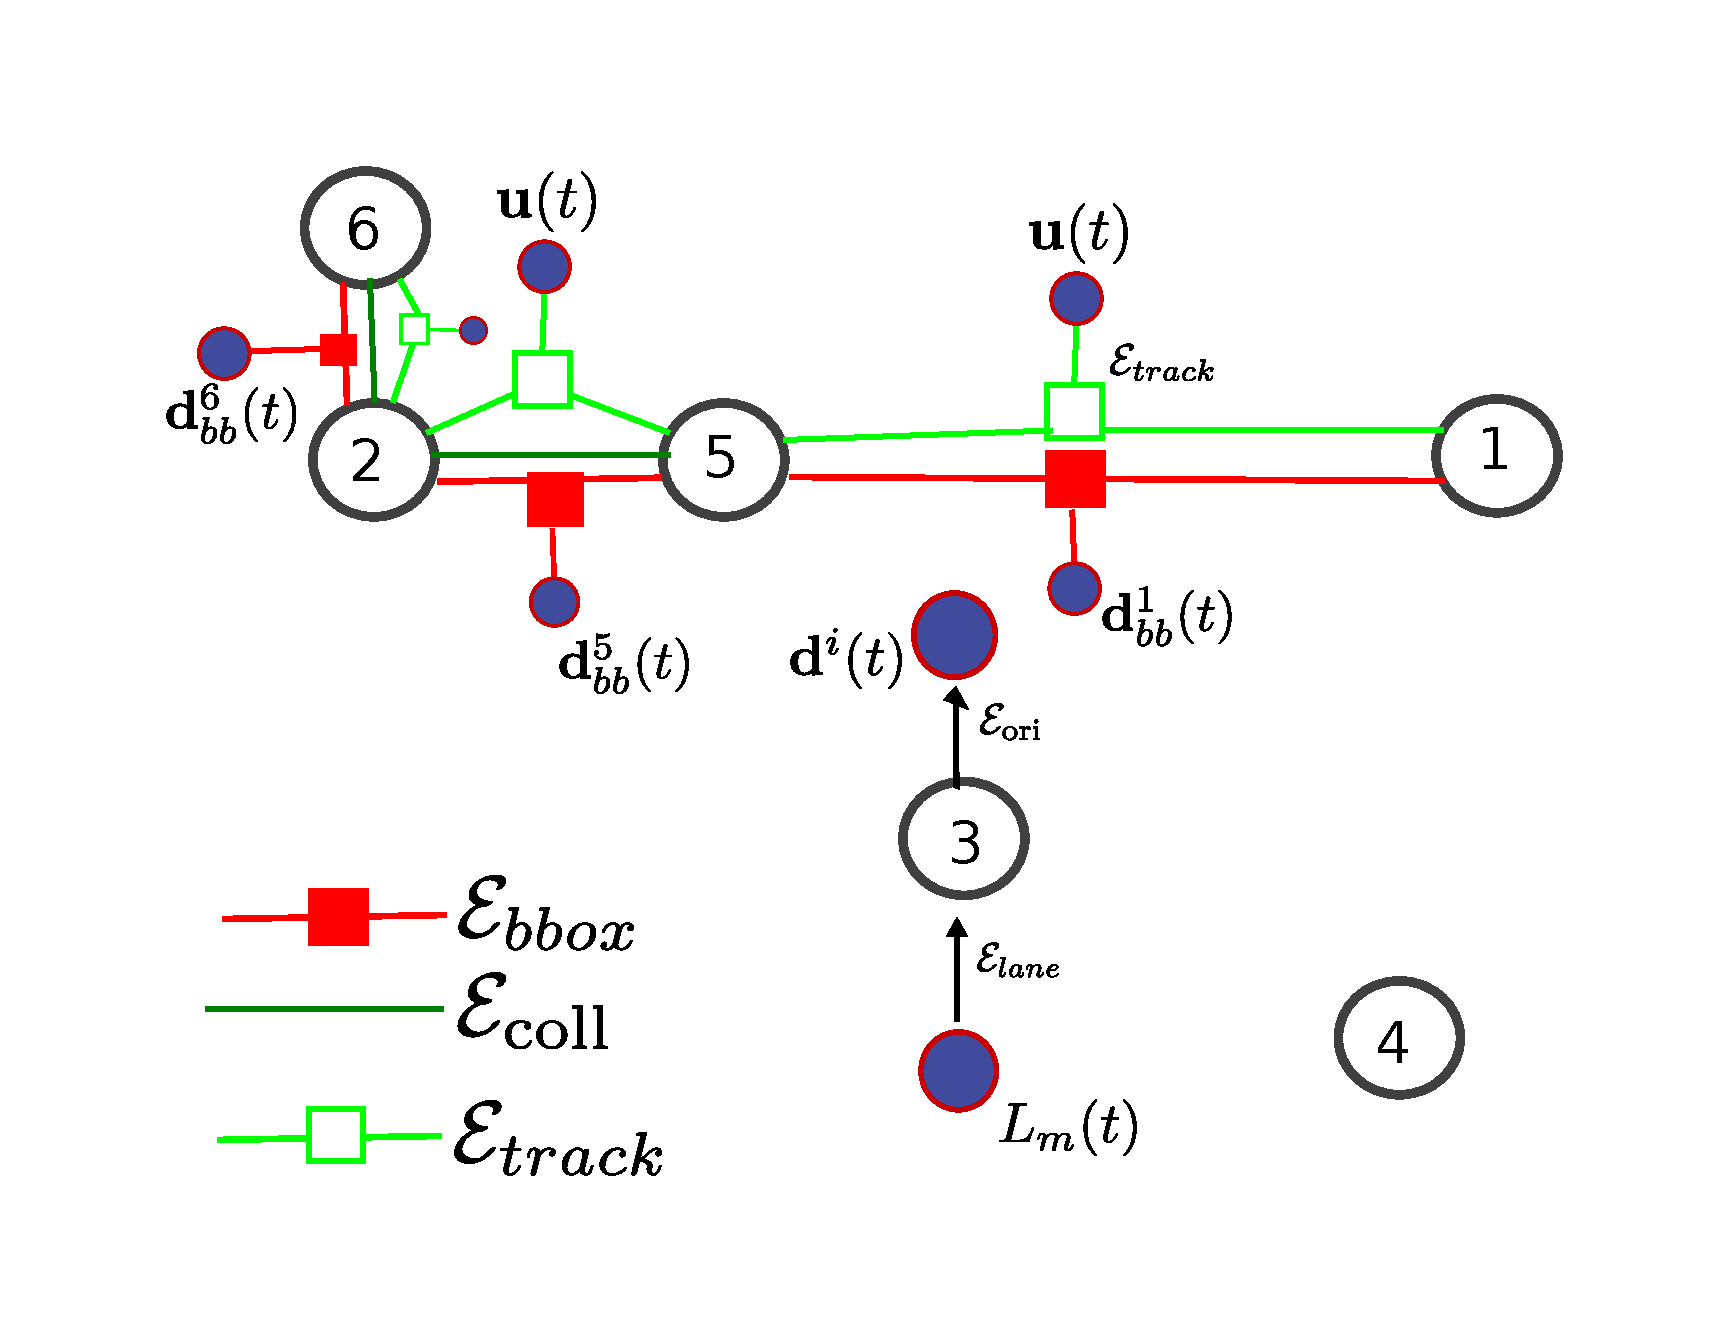
\includegraphics[width=\columnwidth]{graphics/graphicalModelFrom61ConstVars.pdf}
  \caption{Graphical model. The six numbered black circles represent the
    unknown state variables of each car. All other nodes in the graphical model
    are assumed
    observed variables. Consider each energy in the model one by one. (1)
    Bounding box energy: The bounding box energy without occlusion modeling is
    a unary term, but with occlusion it becomes a higher order term that
    affects the state of occluder as well. In this graphical model we assume
    that the scene is being observed from left to right, hence "2" occludes "6"
    and "5" and "5" occludes "1". The bounding box detection is represented by
  $\mathbf{d}_{bb}^i(t)$ and the statistical dependencies are represented by
  red lines. (2) Point tracks ($\Energy{track}$): Since occlusion is also
  included in modeling point tracks energy we have similar interdependencies
  for point tracks energy. The available point tracks are modeled by
  $\mathbf{u}(t)$. (3) Collision ($\Energy{coll}$) : The collision energy
  mathematically is a dense graph between all the TP but here we represent
  collision among only those TP that are near enough to have a significant
collision energy. (4) Orientation from detection ($\Energy{ori}$) (5) Orientation from lane (and map) information ($\Energy{lane}$)}
  \label{fig:graphmodel}
\end{figure}

\section{Related Work}
TODO:
\vfill
\pagebreak
Related work continued
\vspace{15cm}

\section{Problem Definition}
TODO:
\vspace{4cm}


\section{Notation}


\begin{table}[h]
  \begin{tabular}{|l|l|}
    \hline
    Symbol & Meaning \\
    \hline
    $\pos{i}{t}$ & Position of $i$th car at time $t$\\
    $\ori{i}{t}$ & Orientation of $i$th car at time $t$\\
     $\dimsn{i}$ & 3D bounding box of the car (dimensions)\\
    $\state{i}{t}$ & State of car $=\{\pos{i}{t}, \ori{i}{t}, \dimsn{i}\}$\\
    $\egop$ & Position of camera at time $t$\\
    $\egoo$ & Orientation of camera at time $t$\\
    $\relp{i}{t}$ & Relative car pose w.r.t. camera \\
    $\tracklets$ & 3D points tracked on car $i$ in its own frame\\
    $\trackp{t}$ & Projection of $\tracklets$ in camera\\
    $\projectionOf{.}$ & Projection function for pose $\relp{i}{t}$\\
    $\bb{i}$ & 2D bounding box of the car in image\\
    \hline
  \end{tabular}
\end{table}

%%%%%%%%% BODY TEXT
\section{The Model}

The objective is to find the most likely traffic participant (TP) state given
various evidences $\mathbb{E} = \{\{\trackp{t}\}, \{\bb{i}\}, \text{lane det.},
\text{map}, \text{GPS}\}$.

Mathematically, find:
\begin{align}
  \{\state{i}{t}\}^* &= \arg \max P(\{\state{i}{t}\} | \mathbb{E})
\end{align}

Bayes rule
\begin{align}
  P(\{\state{i}{t}\} | \mathbb{E}) &=
  \frac{1}{Z}P( \mathbb{E} | \{\state{i}{t}\})P(\{\state{i}{t}\})
\end{align}


Assume conditional independence according to graphical model in
\ref{fig:graphmodel}.

\begin{multline}
  P(\{\state{i}{t}\} | \mathbb{E}) =
  \frac{1}{Z}
  \prod_{t=s_i}^{e_i}\prod_{i,j: i \ne j}(P(\state{i}{t}, \state{j}{t}))\\
%
  \prod_{i=1}^{N}
  \prod_{t=s_i}^{e_i}
  P(\bb{i} | \state{i}{t})
  P(\trackp{t} | \state{i}{t})\\
  P(\state{i}{t} | L_m(t))
  P(\state{i}{t} | \state{i}{t-1})
  P(\state{i}{t})
\end{multline}

We can formulate similar objective function in negative log domain:
\footnote{TODO:Resolve inconsistency in summation absorption in energy terms.}
\begin{multline}
  -\log{P(\{\state{i}{t}\} | \mathbb{E})} = 
  Z' + \sum_{i,j:i\ne j} \sum_{t=s_i}^{e_i}  \WEnergyCol \\
  + \sum_{i=1}^N \sum_{t=s_i}^{e_i}
    \WEnergy{box}
  + \WEnergy{track}\\
  + \WEnergy{lane}
  + \WEnergy{dyn}
  + \WEnergy{prior}
\end{multline}

\section{Modeling traffic participants}
\label{sec:TPmodel}
Following standard model of occupancy in 3D reconstruction community, we model
the TP's as high occupancy regions in space. We model the
uncertainty in occupancy equivalent of transparency i.e. the regions that are
more certain to be occupied are viewed as relatively more opaque then other
regions. Based on this intuition we model TP's translucent
ellipsoids whose opacity is maximum at the center and drops off away from the
center. More specifically we model, the occupancy of a TP as a
logistic function, 

\begin{align}
   \occf = L(\mathbf{x}; \pos{i}{t}, \Sigma_i)
\end{align}
where $L(.)$ is the logistic function defined by
\begin{align}
  L(\mathbf{x}; \pos{i}{t}, \Sigma_i) = \frac{1}{
    1 + e^{-k(1 - d(\mathbf{x},\pos{i}{t}))}
    }
\end{align}
where $d(\mathbf{x},\pos{i}{t}) =
(\mathbf{x}-\pos{i}{t})^\top\Sigma_i(\mathbf{x}-\pos{i}{t})$ and $k =
10\ln{49}$. $k$ is chosen such that $L(.) = 0.98$ when $d(.) =
0.9$. $\Sigma_i$ determines the spread of the ellipsoid and depends on the
dimensions of the TP. Please refer to supplementary material 
for computation of $\Sigma_i$ from TP's dimensions.

We model the probability of a point $\mathbf{x}_j$ on a object $i$ getting successfully
observed in a camera image at point $\trackpj{t}$ is dependent up two factors,
(1) reflection and (2) transmission through intermediate space. The reflection
part ensures that there is an object to reflect a point at a certain region in
the 3D space while transmission part models occlusion.
\begin{align}
  P^{(ij)}_{\text{observation}} = P^{(ij)}_{\text{reflection}}P^{(j)}_{\text{transmission}}
\end{align}

%%%%%%%%%%%%%%%%%%%%%%%%%%%%%%%%%%%%%%%%%%%%%%%%%%%%
\subsection{Reflection probability}
For Lambertian reflection we replace the surface normal with the
gradient of occupancy.
%
\begin{align}
  \Prefl = (\max \{0, \nabla \occf^\top
  \hat{\mathbf{r}_j}\})^2
\end{align}
%
where $\ray =
\frac{K^{-1}\trackpj{t}}{\|K^{-1}\trackpj{t}\|}$ is unit vector in the
direction of ray. The gradient in the direction opposite to ray yields -ve
probability which needs to be clipped off. Squaring the function keep it
smooth near zero.

%%%%%%%%%%%%%%%%%%%%%%%%%%%%%%%%%%%%%%%%%%%%%%%%%%%%
\subsection{Transmission probability}
A model for transmission of light through a material of thickness $x$,
density $\rho$ and opacity $k_o$ is given by Beer-Lambert law 
%
\begin{align}
  I(x) = I_0e^{-k_o\rho x}
\end{align}
%

Since both opacity and density are represented by the occupancy function
$\occftot = \sum_i \occf$, and also the domain of our $\occftot$ is $[0, 1]$ instead of $[0,
\infty]$ as in case of $k_o$; we replace $e^{-k_o\rho}$ by the transparency
function $1 - \occftot$. So the transmission probability over a small distance
$d\lambda$ is given by
%
\begin{align}
  P_{\text{transmission}}(\lambda + d\lambda) =
  P_{\text{transmission}}(\lambda) (1-\occftot)^{d\lambda}
\end{align}
%

For a given 3D point $\mathbf{x}_j = \lambda \ray$, the probability that the
point $\trackpj{t}$ is reflected from a distance $\lambda$ is given by

\begin{align}
  %P^{(j)}_{\text{observation}}(\lambda) &= P_{\text{reflection}}
  \Ptrans &=
  \prod_{0}^{\lambda} (1 - \occft{\lambda \ray})^{d\lambda} %\\
  %= \max \{ 0, (\nabla f_{occ}&(\lambda \ray)^\top \ray) \}
  %\prod_{0}^{\lambda} (1 - f_{occ}(\lambda \ray))^{d\lambda}
  \label{eq:ptrans-integral}
\end{align}
where $\prod_{0}^{\lambda}$ represents the \emph{product integral} from $0$ to
$\lambda$. 

In practice, the integral for transmission probability
\eqref{eq:ptrans-integral} is difficult to compute even numerically. So we
choose a product of sigmoid function that approximates the behaviour of
transmission probability,
%
\begin{align}
\label{eq:evalCumulativePtrans}
  \Ptrans &= \prod_i L_u(\trackp{t}; \muiu,\Sigmaiu)L_{\lambda}(\lambda; \mu^i_d)
\end{align}
%
where $L_u(.)$ is sigmoid in image domain with $\mu^i_u$ and $\Sigma^i_u$
representing the elliptical projection of $i^{th}$ TP.
$L_{\lambda}(.)$ is sigmoid in the depth domain with $\mu^i_d$ as the mean
depth of the $i^{th}$ TP.
%
\begin{align}
  L_u(\mathbf{u}; \muiu,\Sigmaiu) &= \frac{1}{
    1 + e^{-k_u(1 - (\mathbf{u} - \muiu)^\top\Sigmaiu(\mathbf{u} -
    \muiu))}
  }
  \\
  L_{\lambda}(\lambda; \mu^i_d) &= \frac{1}{
    1 + e^{-k_d(\lambda - \mu^i_d)}
}
\end{align}
%

\begin{comment}%% Comment
  A product integral is a simple integral in log domain
  \begin{align}
    \prod_{0}^{\lambda} (1 - f_{occ}(\lambda \ray))^{d\lambda} =
    e^{\int_{1}^{\lambda} \ln{(1 - f_{occ}(\lambda \ray))}{d\lambda}}
  \end{align}
\end{comment}%% Comment


%%%%%%%%%%%%%%%%%%%%%%%%%%%%%%%%%%%%%%%%%%%%%%%%%%%%
\section{Energies}
%%%%%%%%%%%%%%%%%%%%%%%%%%%%%%%%%%%%%%%%%%%%%%%%%%%%
We explain energies in this section

%%%%%%%%%%%%%%%%%%%%%%%%%%%%%%%%%%%%%%%%%%%%%%%%%%%%
\subsection{Point tracks energy with occlusion}
\label{sec:totalContPtTracksEnergy}
We model continuous point tracks energy with explicit occlusion reasoning as
the expected re-projection error over the association probability,

\begin{multline}
  \Energy{traci}(\{ \relp{i}{t} \}_i, \{ \relp{i}{t-1} \}_i, \{\dimsn{i}\}_i ) = \\
    \sum_{i=1}^{N} 
    %\sum_{t = s_i}^{e_i}
    \sum_{j = 1}^{M}
    \int_1^\infty \assocP\Ereproj(\lambda) d\lambda
\end{multline}
where $\assocP$ is the association probability of
$j$\textsuperscript{th} point with $i$\textsuperscript{th} TP at depth $\lambda$
and $\Ereproj(\lambda)$ is the re-projection error given by
%
\begin{align}
  \assocP &= \Prefl\Ptrans\\
  \Ereproj(\lambda) &= \left\|\trackpj{t+1} - \projectionOft{\invProjectionOf{\trackpj{t}, \lambda}}\right\|^2 .
  \label{eq:reprojerror}
\end{align}

The  $\projectionOf{.}$ and $\invProjectionOf{.}$ denote the projection and
inverse projection functions that project 3D point to camera image and vice
versa. Note that inverse projection $\invProjectionOf{.}$ depend on both the
point $\trackp{t}$ and the unknown depth $\lambda$. Also note that the inverse projection is dependent on TP pose at time $t$ while the projection depends on pose at time $t+1$ which can be different.

\begin{comment}
  \subsubsection{Occupancy function}
  Assuming occupancy to be a
  probability distribution over 3D space. For each TP the
  occupancy is modeled as a logistic function 
  \begin{align}
     \occf = L(\mathbf{x}; \pos{i}{t}, \Sigma_i)
  \end{align}
  where $L(.)$ is the logistic function defined by
  \begin{align}
    L(\mathbf{x}; \pos{i}{t-1}, \Sigma_i) = \frac{1}{
      1 + e^{-k(1 - d(\mathbf{x},\pos{i}{t-1}))}
      }
  \end{align}
  where $d(\mathbf{x},\pos{i}{t-1}) =
  (\mathbf{x}-\pos{i}{t-1})^\top\Sigma_i(\mathbf{x}-\pos{i}{t-1})$ and $k =
  10\ln{49}$. $k$ is chosen such that $L(.) = 0.98$ when $d(.) =
  0.9$
  % Once we have our distribution over $\lambda$, $\lambdadist$ we can compute the
  % reprojection of $\trackpj{t-1}$ over image in time $t$ as a function of
  % $\lambda$. Let
\end{comment}


\begin{comment}
  \subsubsection{Approximations}
  Reflection probability of $i$th TP is easy to compute
  analytically 
  \begin{multline}
    \Prefl =
    (\max \{ 0, \nabla \occf^\top \ray \})^2 \\
    = (\max \{ 0, \nabla \occfxi^\top\ray \})^2
    \label{eq:analytic-prefl}
  \end{multline}
  where 
  \begin{multline}
    \nabla \occfxi^\top\ray \\=
    \nabla k\dishort \sech^2\left(\frac{k}{2}\dishort\right)
  \end{multline}
  where $\dishort = 1-d(\mathbf{x}, \pos{i}{t-1})$ is a signed distance measure
  from the contour of the ellipsoid where $d(\mathbf{x}, \pos{i}{t-1})$ is 1.

  However, the transmission probability needs to be approximated.  
  %
  % \subsubsection{Computing $\Prefl$ and $\Ptrans$}
  % Focusing on  $\nabla \occfxi$ 
  % 
  % \begin{multline}
  %   \nabla \occfxi =\\
  %   \frac{-k\nabla d(\mathbf{x}, \pos{i}{t-1})e^{-k(1-d(\mathbf{x}, \pos{i}{t-1}))}}{
  %     (1 + e^{-k(1-d(\mathbf{x}, \pos{i}{t-1}))})^2
  %   } \\ 
  %   = -k\nabla d(\mathbf{x}, \pos{i}{t-1})\sech^2\left(\frac{k}{2}(1-d(\mathbf{x},
  %   \pos{i}{t-1}))\right)
  %   \\
  %   = \nabla k\dishort \sech^2\left(\frac{k}{2}\dishort\right)
  % \end{multline}
  % where $\dishort = 1-d(\mathbf{x}, \pos{i}{t-1})$ is a signed distance measure
  % from the contour of the ellipsoid where $d(\mathbf{x}, \pos{i}{t-1})$ is 1.
  % Focusing on $\nabla d(.)$
  % 
  % \begin{align}
  %   \nabla d(\mathbf{x}, \pos{i}{t-1}) = 2\Sigma_i(\mathbf{x} - \pos{i}{t-1})
  % \end{align}
  % Back to \eqref{eq:analytic-prefl}
  % 
  % \begin{multline}
  %   (\max \{ 0, \nabla \occf^\top \ray \})^2 = \\
  %   \sech^4\left(\frac{k}{2}\dishort\right) 
  %   (\max \{ 0 , \nabla k\dishort^\top\ray\})^2
  % \end{multline}
  % 
  % The probability is simply $\sech^2(.)$ scaled by gradient of ellipsoid
  % $\nabla k\dishort$ projected in the ray direction $\ray$.
  % 
  % \begin{align}
  %   \Ptrans = 
  %   e^{\int_{1}^{\lambda} \ln{(1 - f_{occ}(\lambda \ray))}{d\lambda}}
  % \end{align}
  % \begin{multline}
  % \int_{1}^{\lambda} \ln{(1 - f_{occ}(\lambda \ray))}{d\lambda}
  % =  \\
  % \int_{1}^{\lambda} \ln{\left(1 - \sum_i \occfi\right)}{d\lambda}
  % \end{multline}
  % 
  % The above integral is very difficult to approximate or compute analytically.
  So based on intuition, we approximate the $\Ptrans$ by following function
  \begin{align}
  \label{eq:evalCumulativePtrans}
    \Ptrans &= \prod_i L_u(\mathbf{u}, \mu^i_u,\Sigma^i_u)L_{\lambda}(\lambda; \mu^i_d)\\
    L_u(\mathbf{u}, \mu^i_u,\Sigma^i_u) &= \frac{1}{
      1 + e^{-k_u(1 - (\mathbf{u} - \mu^i_u)^\top\Sigma^i_u(\mathbf{u} -
      \mu^i_u))}
    }
    \\
    L_{\lambda}(\mathbf{u}, \lambda; \mu^i_d) &= \frac{1}{
    1 + e^{-k_d(\lambda - \mu^i_d(\mathbf{u}))}
  }
  \end{align}
  where 
  \begin{align}
    \mu_u^i &= \projectionOf{\pos{i}{t-1}} \label{eq:muiudef}\\
    \Sigma_u^i &= \projectionOf{\Sigma_i} \label{eq:sigmauidef}\\
    \mu^i_d(\mathbf{u}) &= \relp{i}{t}\\
    k_u &= 10\log(49)\\
    k_d &= \frac{\log(49)}{\sqrt{h^2 + l^2 + w^2}}
    \label{eq:ptransmissionInit}
  \end{align}
  is the distance of the centre of the TP from the camera.

  % $\mu^i_d(\mathbf{u}) = \min_{\lambda} d^2_i(\lambda K^{-1}\mathbf{u})$.
  % $\mu^i_d(\mathbf{u})$ is the closest point to the unit contour of ellipsoid.
  % If there are multiple such points, the point closest to the camera is taken as
  % $\mu^i_d(\mathbf{u})$

  The association probability becomes

  \begin{multline}
    \assocP = 
      \sech^4\left(\frac{k}{2}\dishort\right)
      (\max \{ 0, \nabla k\dishort^\top\ray \})^2\\
    \prod_i \Lu
      \Llambda \\
      \label{eq:assocCoeffEval}
  \end{multline}

  So the energy becomes

  \begin{multline}
    \label{eq:integrand}
    \Energy{track}(.) = 
      \sum_{i = 1}^N
      \sum_{j = 1}^{M}
      \int_1^{\infty}
      \assocP
      \Ereproj(\lambda)
      d\lambda
  \end{multline}
  where $x = \lambda \ray$ and $\Ereproj(\lambda) = \|\trackpj{t} -
  f^i_{reproj}(\trackpj{t-1}, \lambda)\|^2$ is reprojection error which is a
  quadratic in $\lambda$

  The integral in the above expression is computed numerically.
\end{comment}

\subsection{Object detection energy with occlusion} 

Object detection is usually followed by non-maximal suppression that results in
discarding similar bounding boxes. When we are jointly optimizing detections
with other cues, it is not usually desirable to go with a single bounding box.
Hence, we keep all the bounding box detections by approximating them with
multi-modal sum of Gaussian like logistic functions. We fit the parametric function of the form 
%
\begin{align}
  S(\bb{i}) = \sum_k A_k \exp(-(\bb{i}-\mu^{(d)}_k)^\top \Sigma^{(d)-1}_k
  (\bb{i}-\mu^{(d)}_k))
\end{align}
%
to detection scores, by non-linear error minimization with initialization from
non-maximal suppressed outputs. Here $\mu^{(d)}_j$ is one of the $k$ modes as a
4D vector representing a single bounding box as $[\minx, \miny, \maxx,
\maxy]^\top$. The optimization is constrained with symmetry and positive
definiteness of $\Sigma^{(d)-1}_k$, $\maxx \ge \minx$ and $\maxy \ge \miny$.

\subsubsection{Detection scores with occlusion reasoning} 
With our model of $\Ptrans$ described in Section \ref{sec:TPmodel}, we can
compute the probability of a point $\mathbf{u}$ on image be occluded assuming
the point is on TP $i$ with mean depth $\mu^{(i)}_d$ as
\begin{align}
  O_{i}(\mathbf{u}, \mu^{(i)}_d) = 1 - \Ptransmud \enspace .
\end{align}

If we a portion of our proposed detection bounding box is known to be occluded,
then we would like to decrease the confidence in the detection score about the
localization of that end of the object. Assuming that the occlusion is often on
the boundary of detection bounding boxes, we want to decrease our confidence on
the mean detection boundaries around the occluded boundaries. 
One of the simplest ways will be to scale the appropriate diagonal element of
$\Sigma_j$ by an appropriate scaling factor proportional to occlusion. But this
does not model appropriate how does occlusion affects the non diagonal terms.
Hence, we choose a covariance addition model where we compute a occlusion
covariance matrix, that provides a measure of occlusion in each direction.


To re-model our detection scores scaled by continuous occlusion we sample
$O_{i}(\mathbf{u}, \mu^{(i)}_d)$ at the hypothesized detection boundaries from
GMM $S(.)$ and we augment the detection boundary covariance matrix by
$\mathcal{P}_{j} = \rho_{j}\rho_{j}^\top$ where $\rho_{j} = O_{j}(\mathbf{u},
\mu^{(i)}_d)$. The new covariance matrix in detection score is given by 
%
\begin{align}
  \Sigma'^{(d)}_j = \mathcal{P}_{j} + \Sigma^{(d)}_j
\end{align}
%
The detection scores GMM with occlusion is given by replacing the covariance
matrix
%
\begin{multline}
  S'(\bb{i}) =\\
  \sum_j A_j \exp(-(\bb{i}-\mu^{(d)}_j)^\top \Sigma'^{(d)-1}_j
  (\bb{i}-\mu^{(d)}_j))
\end{multline}

The energy of detection scores is simply take to be the inverse of the detection score.
\begin{align}
  \Energy{detect}(\{ \relp{i}{t} \}_i, \{ \relp{i}{t-1} \}_i, \{\dimsn{i}\}_i ) = \frac{1}{S'(\bb{i})}
\end{align}

\subsection{Lane energy}
\label{sec:laneEnergy}
 The lanes are modeled as splines. Here we assume that the confidence in lane
 detection is decreases as the distance from the lane center increases.  The
 energy is given by the dot product between car orientation and tangent to the
 lane at that point.

\begin{multline}
  \label{eq:laneOrientationEnergy}
  \Energy{lane} = \\
  \sum_{m \in M_{\text{close}}}
  (1 - \ori{i}{t} \cdot \text{TAN}(L_{m}(k), \pos{i}{t}) )
\LaneUncertainty{\pos{i}{t}}
\end{multline}
where $M_{\text{close}} = \{m : \text{DIST}(L_{m}(k), \pos{i}{t}) < 50\} $ is
the set of nearby lanes and 
\begin{multline}
\LaneUncertainty{\pos{i}{t}} = \\
  \frac{1}{1 + exp(-q(w_{\text{road}} - \text{DIST}(L_{m}(k), \pos{i}{t})))}
\end{multline}
for some constant $w_{\text{road}}$ that represents the width of the road.

\subsection{Transition probability}
Dynamics constraints should not only enforce smooth trajectories, but also the
holonomic constraints.  The following energy adds a penalty if the change in
position is not in direction of previous orientation.

\begin{align}
  \label{eq:totalPosTransitionEnergy}
  \Energy{dyn-hol} = 1 - \ori{i}{t-1} \cdot (\pos{i}{t} - \pos{i}{t-1})
\end{align}

The following energy adds a penalty for change in position and orientation
but a penalty for change in velocity is much better approximation. However, in
a Markovian setting that would mean extending the state space of the car to
include velocity.

\begin{align}
  \Energy{dyn-ori} &= \|\ori{i}{t} - \ori{i}{t-1}\|^2\\
  \Energy{dyn-vel} &= \|(\pos{i}{t} - 2\pos{i}{t-1}) + \pos{i}{t-2}\|^2
\end{align}

As a result the dynamics are modeled by weighted combination of holonomic
constraint and smoothness constraints.

\begin{align}
  \WEnergy{dyn} &= \WEnergy{dyn-hol} + \WEnergy{dyn-ori} + \WEnergy{dyn-vel}
\end{align}

 
\subsection{Collision energy}

Bhattacharya coefficient $\int_a^b\sqrt{p(x)q(x)}dx$ is a measure of similarity
of two distributions $p(x)$ and $q(x)$. If we represent TPs as gaussians in
Birds eye view (BEV), then similarity is a measure of collision. Exactly
overlapping distribution results in coefficient as 1. 
%The analytical form of
%Bhattacharya coefficient has been taken from
%\url{http://like.silk.to/studymemo/PropertiesOfMultivariateGaussianFunction.pdf}

\begin{multline}
  \label{eq:collisionEnergyHellingerDistance}
  \EnergyCol =\\ -\log\left(
  A_{ij}
  e^{-\frac{1}{8}
    \left(\pos{i}{t} - \pos{j}{t}\right)^\top
    P^{-1}
    \left(\pos{i}{t} - \pos{j}{t}\right)
    }
    \right)
\end{multline}
where 
\begin{align}
  A_{ij} &= \frac{|\Sigma_i|^\frac{1}{4}|\Sigma_j|^\frac{1}{4}}
  {|P|^\frac{1}{2}}\\
  P &= \frac{1}{2}\Sigma_i + \frac{1}{2}\Sigma_j\\
\Sigma_i^{-1} &= R^\top_{\ori{i}{t}} \begin{bmatrix} 2/l_i & 0 \\ 0 & 2/w_i \end{bmatrix}
R_{\ori{i}{t}}
\end{align}


\subsection{Size Prior}

Prior can include among many other things the size prior on the car.

\begin{align}
  \label{eq:totalSizeEnergy}
  \Energy{prior} &= (\dimsn{i} - \expDimsn)^\top\Sigma_{\expDimsn}^{-1}(\dimsn{i} -
  \expDimsn)
\end{align}

where $\expDimsn$ is the mean TP dimensions and
$\Sigma_{\expDimsn}$ is the correspondence covariance matrix.

%%%%%%%%%%%%%%%%%%%%%%%%%%%%%%%%%%%%%%%%%%%%%%%%%%%%
\section{Association error evaluation}

To verify the correctness of our association probability $\assocP$ we perform
association error experiment that compare the accuracy of point track
association with TPs with that of bounding box baseline method.

% \begin{align}
%   f^{i}_{reproj}&(\trackpj{t-1}, \lambda) =
%   \projectionOf{\invProjectionOf{\trackpj{t-1}}}\\
%   %&= K(R^i_t ((R^i_{t-1})^\top\lambda \ray - (R^i_{t-1})^\top T_{t-1}) + T_{t})\\
%   &= \frac
%   {p_{1:2}\lambda + q_{1:2}}
%   {p_{3}\lambda + q_{3}}
% \end{align}
% where $p_{1:3} = KR^i_t(R^i_{t-1})^\top\ray$ and
% $q_{1:3} = KR^i_t(R^i_{t-1})^\top T_{t-1} + KT_t$
% 
% Now that we have an association from TP $i$ to point track $j$ through
% $\lambda$, we can come up with an association probability
% \begin{align}
%    \assocP &= \frac{(\max \{ 0, \nabla \occf^\top
% \ray \})^2 }{P_{\text{reflection}}}\lambdadist\\
% &=(\max \{ 0, \nabla \occf^\top \ray \})^2
%   \prod_{0}^{\lambda} (1 - f_{occ}(\lambda \ray))^{d\lambda}
% \end{align}

Note that the fraction $\assocP$ although called association probability does
not capture the entire information that we have available for compute
association of points to tracks. This above fraction is the association
probability given the hypothesized parameters of TP model. 

To compute the association probability between TP $i$ and
point track $j$ we must use re-projection error as well. When the association
$i$ and $j$ is right and the point of reflection is at depth $\lambda$ the
re-projection error must be zero \eqref{eq:reprojerror}, otherwise the error
becomes a measure of distance from the true solution.
The error terms can be converted to probability domain by considering the error
term as negative log of probability

\begin{align}
  P^{(ij)}_{\text{assoc by reproj}}(\lambda) = \frac{1}{Z}\exp(-\Ereproj(\lambda))
\end{align}

Using both the evidence terms we can write probability of association as
\begin{align}
  P^{(ij)}_{\text{assoc}} = \frac{1}{Z'}\int_0^{\infty} \assocP \frac{1}{\sqrt{2\pi}}\exp(-\Ereproj(\lambda))d\lambda
  \label{eq:prob-assoc}
\end{align}

Once we have the probability of association we can compute the best possible
assignment of TP for each point. The points having very small association
probability are assigned to the background,
\begin{align}
  i^*_{j} = \argmin_{i} \int_0^\infty \assocP \Ereproj(\lambda) d\lambda
\end{align}

We use bounding box based assignment of point tracks to TPs as the baseline.
For the regions where the bounding boxes overlap, we assign the points to the
TP that has smaller mean depth then the competing bounding box.

{\small
\bibliographystyle{ieee}
\bibliography{model}
}
\end{document}
